\section{Methodology}

In this section, we first formalize the problem in Section~\ref{sec:formulation}. Next, we elaborate on the design of \our in Section~\ref{sec:method_design}. Finally, we introduce the process for training a dedicated orchestrator in Section~\ref{sec:learnable}. Figure~\ref{fig:piepine} provides an overview of our methodology.

\begin{figure*}[t]
    \centering
    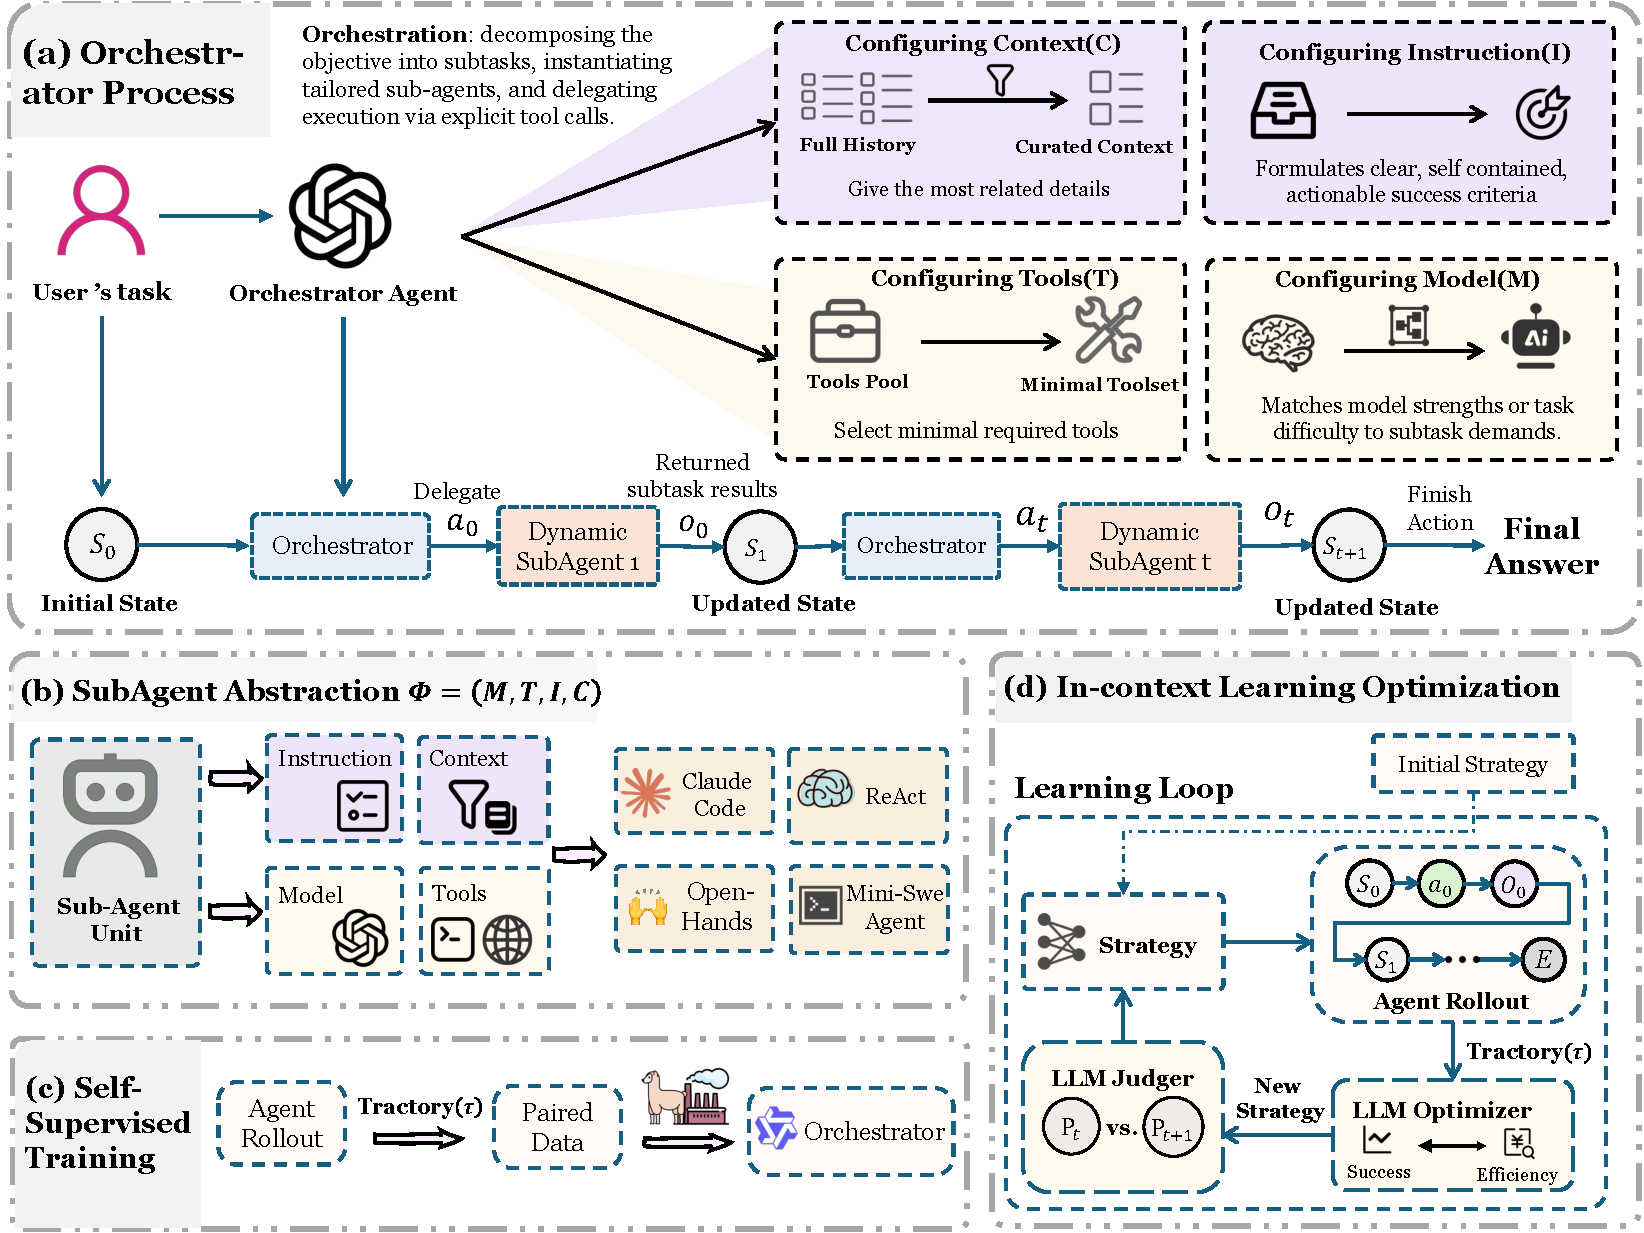
\includegraphics[width=\textwidth]{figures/introduction.pdf}
    \caption{Overall design of our proposed agentic framework, \our{}, for complex, long-horizon tasks. The orchestrator solves a user task by repeatedly delegating subtasks to on-the-fly instantiated sub-agents, each defined by a unified four-tuple $(I,C,T,M)$. The orchestrator is learnable and can improve its decomposition, context routing, and capability allocation from past experience.}
    \label{fig:piepine}
\end{figure*}


\subsection{Problem Formulation}
\label{sec:formulation}
In this paper, we mainly focus on solving complex agentic tasks. The agentic system solves a user goal $G$ through multi-step interaction with an environment.
The environment exposes an \emph{environment-level} action space $\mathcal{A}_{\text{env}}$ (e.g., shell commands, web operations, code edits) and returns feedback such as observations, tool outputs, and error messages.
An interaction trajectory for a task can be therefore defined as:
\[
\tau = (s_0, a_0, o_0, s_1, a_1, o_1, \dots, s_T),
\]
where $s_t \in \mathcal{S}$ denotes the system state at step $t$ (including accumulated history, intermediate results, and environment feedback), $a_t$ is the action taken at step $t$, and $o_t \in \mathcal{O}$ is the returned observation.
The system evolves according to a state-transition function
\[
s_{t+1} = \delta(s_t, a_t, o_t),
\]
where $\delta: \mathcal{S} \times \mathcal{A}_{\text{env}} \times \mathcal{O} \rightarrow \mathcal{S}$ maps the current state, action, and observation to the next state by incorporating newly returned information into the system's internal state.

\paragraph{Sub-agent-as-tools view.}
We focus on the sub-agent-as-tools paradigm, where a \emph{main agent} (orchestrator) can either act in the environment directly or delegate a subtask to a sub-agent as a tool call.
Accordingly, the orchestrator operates over a \emph{system-level} action space that typically includes three types of actions:
(1) environment actions $u \in \mathcal{A}_{\text{env}}$,
(2) delegation actions (\texttt{Delegate}$(\cdot)$) that invoke a sub-agent to execute,
and (iii) termination (\texttt{Finish}).
We denote this generic orchestration action space as
\[
\mathcal{A}_{\text{orch}} \supseteq \mathcal{A}_{\text{env}} \ \cup\ \{\texttt{Delegate}(\cdot),\ \texttt{Finish}(y)\}.
\]
Different systems mainly differ in how \texttt{Delegate} is parameterized (e.g., delegating with only context vs.\ delegating to a fixed set of roles), and in whether the orchestrator itself also performs environment actions.

Our objective is to maximize task success, optionally trading off execution cost:
\[
\max_{\pi}\ \mathbb{E}\Big[\mathbf{1}\{\text{Success}(G)\}-\lambda\cdot \text{Cost}(\tau)\Big],
\]
where $\pi$ is the orchestrator policy, $\text{Cost}(\tau)$ may include token usage, tool calls, latency, or monetary cost, and $\lambda$ controls the cost--performance trade-off.


\subsection{\our{} }
\label{sec:method_design}

\paragraph{A unified four-tuple agent abstraction.}
\our{} models \emph{both} the main agent and sub-agents under a unified framework-agnostic abstraction.
We define an agent instance as an instantiable four-tuple
\[
\Phi = (I, C, T, M),
\]
where $I$ is the task instruction specifying the current objective and success criteria,
$C$ is the curated working context the agent conditions on,
$T$ is the tool set defining the agent's action space,
and $M$ is the underlying model that interacts with the environment.
This abstraction explicitly separates two complementary axes that require \textit{specialization}:
\emph{working memory} $(I,C)$ and \emph{capabilities} $(T,M)$.
Notably, we do not view a sub-agent as a static entity, but rather as a \emph{dynamic} unit that can be parametrized and created at runtime. 

The main agent (orchestrator) can also be represented by a tuple
$\Phi^{\text{main}}=(I^{\text{main}},C^{\text{main}},T^{\text{main}},M^{\text{main}})$.
The difference is that $T^{\text{main}}$ exposes \emph{system tools} for orchestration (e.g., \texttt{Delegate}, \texttt{Finish}) rather than environment tools in $\mathcal{A}_{\text{env}}$.

\paragraph{Action Space of Orchestrator.}
Building on this abstraction, \our{} decouples orchestration from execution.
The orchestrator in \our{} never directly takes environment actions in $\mathcal{A}_{\text{env}}$.
Instead, it operates only the two following actions:
\[
\mathcal{A}_{\our} = \{\texttt{Delegate}(\Phi),\ \texttt{Finish}(y)\}.
\]
At step $t$, the orchestrator samples an action $a_t \in \mathcal{A}_{\our}$.
If $a_t=\texttt{Delegate}(\Phi_t)$, it spawns an executor $A(\Phi_t)$ to execute the subtask and returns an observation $o_t$.
If $a_t=\texttt{Finish}(y)$, the interaction terminates with the final answer $y$.
Returned observations are integrated into the next state via $s_{t+1}=\delta(s_t,a_t,o_t)$.

\paragraph{Implementation of \texttt{Delegate} and \texttt{Finish}.}
We implement \our{} with two system tools available to the Orchestrator: \texttt{Delegate} and \texttt{Finish}.
\texttt{Delegate} takes $\Phi_t=(I_t,C_t,T_t,M_t)$ as arguments and instantiates an executor accordingly.
The executor runs with model $M_t$, is restricted to the tool set $T_t$, and conditions only on $(I_t,C_t)$.
It returns a structured observation $o_t$ to the Orchestrator, typically including (i) a concise result summary, (ii) relevant artifacts (e.g., files, references), and (iii) error messages or logs if execution fails.
\texttt{Finish} terminates the interaction and outputs the final response $y$.

\paragraph{Advantages of \our{}}
Our proposed \our{} offers several key advantages.
First, it dynamically equips each sub‑agent with tailored capabilities on demand, which substantially improves the accuracy of task execution. Unlike prior works~\cite{sun2025scaling, anthropic_claude_code_subagents}, the orchestrator deliberately provides well‑structured context for the sub‑agent to use. As shown later in Section~\ref{sec:adv1}, this careful context management enhances the model’s ability to solve tasks.
Second, the orchestrator operates solely on a four‑tuple abstraction and remains independent of the internal implementation of sub‑agents. This flexibility allows us to employ various designs for sub‑agents, such as a simple React approach~\cite{yao2022react} or a mini‑SWE agent.
Third, the orchestrator can learn from extensive experience. We will then detail this in Section~\ref{sec:learnable}. These learnable aspects include basic task orchestration skills (i.e., what to do, what to condition on, and which tool to use) as well as advanced features (e.g., adaptive model routing, where the goal might be to balance performance and cost by selecting the most suitable model).


% \paragraph{Context routing and configuration knobs.}
% Full-parameterized delegation exposes explicit control over what is delegated \emph{and} how it is executed.
% Concretely, the Orchestrator configures (i) the \emph{work package} $(I_t, C_t, T_t)$---a self-contained instruction, a task-sufficient curated context, and a minimal tool subset---and (ii) the \emph{model routing} choice $M_t$ from a model pool.
% In practice, we keep $T_t$ minimal to reduce tool-induced context overhead, and defer cost--performance trade-offs to the routing policy over $M_t$ (Section~\ref{sec:learnable}).



\subsection{Learnable Orchestrator}
\label{sec:learnable}

With $\mathcal{A}_{\our}={\texttt{Delegate}(\Phi),\texttt{Finish}(y)}$, the orchestration task can be expressed as learning a policy over structured actions:
\[
\pi_\theta(a_t \mid s_t),\quad a_t\in\mathcal{A}_{\our}.
\]

In this paper, learning mainly focuses on the two following complementary dimensions:
Since the delegation parameters $\Phi_t=(I_t,C_t,T_t,M_t)$ are explicitly available, learning can focus on two complementary dimensions:
(i) \textbf{Task orchestration}, which determines what to do, what context to use, and which tools to employ.
(ii) \textbf{Model routing}, which selects $M_t$ (the model to call) to balance performance and cost.
In the following, we detail these two learning paradigms.

\paragraph{Supervised fine-tuning (SFT) for task orchestration.}
Given expert orchestration trajectories $\{(s_t,a_t^\star)\}$, we fine-tune the Orchestrator by behavior cloning:
\[
\theta^\star = \arg\max_{\theta}\ \sum_{t} \log p_{\theta}(a_t^\star \mid s_t),
\]
where $a_t^\star$ is the expert action (either $\texttt{Delegate}(\Phi_t^\star)$ or $\texttt{Finish}(y^\star)$).
In our setup, SFT primarily distills \emph{task orchestration}: improving subtask decomposition and the synthesis of $(I_t,C_t,T_t)$, i.e., producing better working memory, and more appropriate tool subsets for each step.
We would like to note that in this work, we prioritize showing the potential of training a specialized orchestrator, thus employing a straightforward SFT approach. Note that others can employ any training methods like GRPO~\cite{shao2024deepseekmath} to improve the task orchestration capability.

\paragraph{Iterative In-context Learning for Cost-aware Orchestration.}
Beyond parameter updates, we also optimize orchestration \emph{without} changing model weights by learning the Orchestrator's \emph{instruction} (prompt) through iterative interaction.
Concretely, we treat the Orchestrator instruction $I^{\text{main}}$ as the learnable object and run \our{} in the environment to collect trajectories
$\tau=\{(s_t,a_t,o_t)\}_{t=0}^{T}$ together with outcome metrics, including task performance and execution cost.
An optimization model then analyzes these trajectories and proposes prompt edits $\Delta I$ to update the instruction:
\[
I^{\text{main}}_{k+1} = \textsc{Optimize}\bigl(I^{\text{main}}_{k},\ \tau_k,\ \text{Perf}(\tau_k),\ \text{Cost}(\tau_k)\bigr),
\]
where $k$ indexes optimization rounds.
By repeatedly rolling out the updated Orchestrator in the environment for $N$ rounds, this process improves cost-aware orchestration behavior (e.g., model compiler/routing decisions and tool usage patterns) and aims to discover Pareto-efficient trade-offs between performance and cost.
